\documentclass[11pt,a4paper]{book}
\textwidth 170 mm
\textheight 250 mm
\topmargin -15 mm
\oddsidemargin -5 mm
\evensidemargin -5 mm

\newcounter{ProblemNo}
\setcounter{ProblemNo}{0}
\def\tempID{0}
%\def\UndAns{} %% <-------------- Uncomment in final version!!
\def\UndAns{\underline}
\def\UndAns{\underline}
\newcommand{\ZOdg}[1]{}
\def\text{}
%\def\dfrac{\displaystyle\frac}

\usepackage{amsfonts,amssymb,amsmath}
\usepackage{graphicx}
\DeclareGraphicsExtensions{.pdf,.PDF,.png,.PNG} % prefer pdf to png
\usepackage{etoolbox}
\usepackage{sidepicture}
\newcommand{\problemID}[3]{\def\tempID{#1 (#3)}\ignorespacesafterend}
%\newcommand{\problemID}[3]{\def\tempID{#1}\noindent{\bf #1, #2}\par}
%\newcommand{\problemID}[3]{\def\tempID{#3: \##1}\par}
%\newcommand{\problemRating}[3]{{\bf #1, #2, #3}\par}
%\newcommand{\problemID}[3]{\def\tempID{\# #1}\par}
%\newcommand{\problemRating}[3]{}
%\newcommand{\xProblem}[8]{#1\par (A) #2\quad (B) #3\quad  (C) #4\quad  (D) #5\quad (E) #6\par Correct: #7\bigskip\bigskip\par }

%\usepackage{xcolor}
%\usepackage{everypage}
%\usepackage[absolute]{textpos}
%\usepackage{rotating}
%\AddEverypageHook{\begin{textblock*}{2.5cm}(0.7cm,5cm)\begin{turn}{90}{\color{red}\Huge\sc Solutions included - do not use for contest}\end{turn}\end{textblock*}}

\newcommand{\Problem}[9]
{%\newpage
%\noindent\addtocounter{ProblemNo}{1}{\bf\arabic{ProblemNo}.\hspace{3pt}~}%
\noindent\addtocounter{ProblemNo}{1}{\bf\tempID.\hspace{3pt}~}%
\edef\answer{{#7}}\def\SettingMode{#8}%
\def\VLine{\vrule height14pt width0pt\quad}#1\nopagebreak\vspace{1ex}\newline%
\VLine\expandafter\ifstrequal\answer{A}{\UndAns{(\rlap{\bf A}\phantom{\bf C})}\ZOdg{A}}{(\rlap{\bf A}\phantom{\bf C})}\nolinebreak\hspace{3pt}%
\ifnum\SettingMode=3{#2}\else\rlap{#2}\fi\quad\ifnum\SettingMode=3\newline\VLine\else\hfil\fi%
\expandafter\ifstrequal\answer{B}{\UndAns{(\rlap{\bf B}\phantom{\bf C})}\ZOdg{B}}{(\rlap{\bf B}\phantom{\bf C})}\nolinebreak\hspace{3pt}%
\ifnum\SettingMode=3{#3}\else\rlap{#3}\fi\quad\ifnum\SettingMode=2\newline\VLine\else\ifnum\SettingMode=3\newline\VLine\else\ifnum\SettingMode=6{\phantom{({\bf C})}\quad\hspace{6pt}\hfil\hfil\newline\VLine}\else\hfil\fi\fi\fi%
\expandafter\ifstrequal\answer{C}{\UndAns{(\rlap{\bf C}\phantom{\bf C})}\ZOdg{C}}{({\bf C})}\nolinebreak\hspace{3pt}%
\ifnum\SettingMode=3{#4}\else\rlap{#4}\fi\quad\ifodd\SettingMode\newline\VLine\else\hfil\fi%
\expandafter\ifstrequal\answer{D}{\UndAns{(\rlap{\bf D}\phantom{\bf C})}\ZOdg{D}}{(\rlap{\bf D}\phantom{\bf C})}\nolinebreak\hspace{3pt}%
\ifnum\SettingMode=3{#5}\else\rlap{#5}\fi\quad\ifnum\SettingMode>1\ifnum\SettingMode<6\newline\VLine\else\hfil\fi\else\hfil\fi%
\expandafter\ifstrequal\answer{E}{\UndAns{(\rlap{\bf E}\phantom{\bf C})}\ZOdg{E}}{(\rlap{\bf E}\phantom{\bf C})}\nolinebreak\hspace{3pt}%
\ifnum\SettingMode=3{#6}\else\rlap{#6}\fi\quad\ifnum\SettingMode=1\hfil\phantom{({\bf C})}\fi\hspace{3pt}\hfil\par\vspace{2ex}\par\noindent{\sc Solution: }#9\bigskip}


\def\TheHead{Junior Finalized}
\makeatletter
\def\ps@pKSF{
\def\@oddfoot{\hfill{\rm \thepage}\hfill}\def\@evenfoot{\hfill{\rm \thepage}\hfill}
\def\@oddhead{\hfill{\em \TheHead}\hfill}\def\@evenhead{\hfill{\em \TheHead}\hfill}
}
\makeatother 
\pagestyle{pKSF}

\begin{document}

\noindent{\large\bf Junior}\bigskip

\noindent\fbox{3 points}\bigskip

\problemID{1}{20257}{Uganda}%
\problemRating{J}{3}{N}%
\Problem{What is the value of $\dfrac{2 \times 0.24}{20 \times 2.4}$?}
{$0.01$}{$0.1$}{$1$}{$10$}{$100$}
{A}{0}
{$\dfrac{2 \times 0.24}{20 \times 2.4} = \dfrac{0.48}{48} = 0.01$}

\problemID{2}{20258}{Switzerland}%
\problemRating{J}{3}{G}%
\Problem{Which square is split up into two pieces that do {\bf not} have the same shape?}
{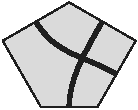
\includegraphics{J02-1}}{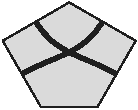
\includegraphics{J02-2}}{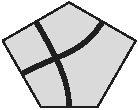
\includegraphics{J02-3}}{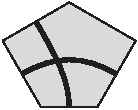
\includegraphics{J02-4}}{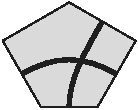
\includegraphics{J02-5}}
{E}{0}
{}

\NSidePictureEPS{J03-1}{\problemID{3}{20259}{Netherlands}%
\problemRating{J}{3}{A}%
\Problem{The number of the dots on opposite faces of a die add to $7$. The vertex labelled $P$ on the die is formed by the faces which have $1$, $2$ and $3$ dots on them. Its vertex sum is the sum of the number of dots on those faces which meet at a given vertex. The vertex sum of $P$ is $1+2+3=6$.\newline
What is the maximum of the vertex sums of vertices $Q$, $R$ and $S$?}
{ $7$}{$9$}{$10$}{$11$}{$15$}
{D}{0}
{The vertex sum of $Q$ is $1+3+5=9$, that of $R$ is $2+3+6=11$ and that of $S$ is $1+2+4=7$.
\newline
Hence the maximum is 11.}}

\NSidePictureEPS[yoffset=-3.5ex,scale=0.8]{J04-1}{\problemID{4}{20260}{Austria}%
\problemRating{J}{3}{N}%
\Problem{A hopping game is played in the following way: Each player hops into the squares, swapping between left foot - both feet - right foot - both feet - left foot - both feet, and so on, as shown. Maya played the game and hopped into exactly $48$ squares starting with her left foot. How many times did her left foot touch the ground?}
{12}{24}{36}{40}{48}
{C}{0}
{Maya's left foot touches the ground in three out of every four steps. Therefore, it touches the ground a total of $\frac 34\cdot 48=36$ times.}}

\NSidePictureEPS{J05-1}{\problemID{5}{20261}{Germany}%
\problemRating{J}{3}{L}%
\Problem{Tim wants to draw the figure shown on a piece of paper, without lifting his pencil off the paper.  The lengths of the lines are given in the figure.  He can choose to start his drawing anywhere.  What is the shortest distance he could draw to complete the figure?}
{$14\ \textup{cm}$}{$15\ \textup{cm}$}{$16\ \textup{cm}$}{$17\ \textup{cm}$}{$18\ \textup{cm}$}
{B}{1}
{The shortest total distance is $3\textup{cm} + 2 \cdot (1\textup{cm} + 2\textup{cm} + 1\textup{cm} + 1\textup{cm}) + 2\textup{cm} = 15\textup{cm}$.}}

\NSidePictureEPS[scale=0.5]{J06-1}{\problemID{6}{20262}{Pakistan}%
\problemRating{J}{3}{G}%
\Problem{The figure shows a square with four circles of equal area, each touching two sides of the square and two other circles.  What is the ratio between the areas of the black region and the grey region?}
{$1:4$}{$1:3$}{$2:3$}{$3:4$}{$\pi:1$}
{B}{0}
{The figure consists of 4 white circles inscribed into a quarter of a square. In each of those quarters, there is one black part and 3  parts of equally big grey area. So the answer is $1:3$.}}

\NSidePictureEPS{J07-1}{\problemID{7}{20263}{Brazil}%
\problemRating{J}{3}{G}%
\Problem{John makes a sequence of structures on a table, beginning with one cube. He makes the next structure by adding five cubes which hide the visible faces of the initial cube, as shown. What is the smallest number of cubes he needs to add to the second structure so that all the visible faces of the second structure are hidden?}
{8}{9}{10}{13}{19}
{D}{0}
{John needs 1 cube on top, 4 cubes to cover 4 faces of the top cube and 8 cube on the ground level. It makes 13 cubes in total.}}

\problemID{8}{20264}{Spain}%
\problemRating{J}{3}{N}%
\Problem{A three-digit palindrome is a number of the form $\text{'}aba\text{'}$ where the digits $a$ and $b$ can either be the same or different. What is the sum of the digits of the largest three-digit palindrome that is also a multiple of 6?}
{16}{18}{20}{21}{24}
{E}{0}
{If it is a multiple of 6, it must be even and its digits must add up to a multiple of three. It must start with 8 to also end in 8, the largest of which is 888 ($8+8+8 =24$).}

\NSidePictureEPS[yoffset=-6.5ex]{J09-2}{\problemID{9}{20265}{Catalonia}%
\problemRating{J}{3}{G}%
\Problem{Martin draws a square with vertices $A$, $B$, $C$, $D$ and a regular hexagon with side $OC$, where $O$ is the center of the square. What is the size of angle $\alpha$?}
{$105^\circ$}{$110^\circ$}{$115^\circ$}{$120^\circ$}{$125^\circ$}
{A}{0}
{Let $E$ be the vertex of the requested angle. Look at the angles of the quadrilateral $OCDE$. \newline
\includegraphics{J09-1} \newline
The angle in $C$ is 45$^\circ$ (angle between side and diagonal of a square). The angle at $D$ is a right angle. The angle at $O$ is 120$^\circ$ (angle of the regular hexagon). Therefore $\alpha = 360^\circ- (45^\circ+90^\circ+120^\circ)= 105^\circ$.}}

\problemID{10}{20266}{Myanmar}%
\problemRating{J}{3}{N}%
\Problem{Ardal encloses a rectangular field with $40\ \textup{m}$ of fence. The side-lengths of the field are all prime numbers.

What is the maximum possible area of the field?}
{$99\ \textup{m}^2$}{$96\ \textup{m}^2$}{$91\ \textup{m}^2$}{$84\ \textup{m}^2$}{$51\ \textup{m}^2$}
{C}{0}
{Perimeter of the fence $40 = 2\cdot(l+w)$, so $l+w=20$.
Both $l$ and $w$ are prime numbers. There are 2 possible pairs $(l,w) =(3,17), (7,13)$.
Maximum possible area is $7\cdot 13 = 91\ \textup{m}^2$}

\noindent\fbox{4 points}\bigskip

\NSidePictureEPS{J11-1}{\problemID{11}{20267}{Netherlands}%
\problemRating{J}{4}{G}%
\Problem{A rectangle is divided into three regions of equal area. One of the regions is an equilateral triangle with side-length $4\ \textup{cm}$, the other two are trapezia, as shown in the figure. \newline
What is the length of the smaller of the parallel sides of the trapezia?}
{$\sqrt2\ \textup{cm}$}{$\sqrt3\ \textup{cm}$}{$2\sqrt2\ \textup{cm}$}{$3\ \textup{cm}$}{$2\sqrt3\ \textup{cm}$}
{B}{0}
{The altitude of the triangle $2\sqrt3$, so its area is $\frac{1}{2}\cdot 4\cdot 2\sqrt3=4\sqrt3$. The area of the rectangle is then $3\cdot 4\sqrt3=12\sqrt3$. Then its length is $\frac{12\sqrt3}{4}=3\sqrt3$. So the length of the smallest parallel side of the trapezia is $3\sqrt3-2\sqrt3=\sqrt3$.}}

\NSidePictureEPS[scale=0.45]{J12-1}{\problemID{12}{20268}{Czech Republic}%
\problemRating{J}{4}{L}%
\Problem{Jelena places the capital letters A, B, C and D into the $2\times 4$ table shown on the right. Exactly one letter is placed in each cell.
She wishes to make sure that in each row and in each $2\times 2$ square, each of the four letters appears exactly once.

In how many ways can she do this?}
{12}{24}{48}{96}{198}
{B}{0}
{The letters A, B, C and D can be arranged freely in the four squares of the first row. There are four options for the first letter, then three options for the second square and two for the third square. That is $4 \times 3 \times 2 \times 1$, which is equal to $24$ options.
\newline
Having filled the first row, consider the second square of the second row. This can't be the letter in the first or third position of the first row. So it must be the same letter as in the fourth position. Therefore the second row is uniquely defined by the first row and there are $24$ options.}}

\NSidePictureEPS{J13-1}{\problemID{13}{20269}{Brazil}%
\problemRating{J}{4}{G}%
\Problem{Sanjay cuts out three circles from three different pieces of coloured card. He places them on top of each other, as shown in Figure 1. He then moves the circles so that all three circles are tangent to each other, as shown in Figure 2.\newline
In the first figure, the area of the visible black region is seven times the area of the white circle.\newline
What is the ratio between the areas of the visible black regions in the two figures?}
{$3:1$}{$4:3$}{$6:5$}{$7:6$}{$9:7$}
{D}{0}
{Let the area of white, black and grey circles respectively be $w$, $b$, $g$. Also if the visible black area in figure 1 are $A_1=b-g=7w$ and in figure 2,  $A_2=b-w-g$ so $A_2=7w-w=6w$ (note that $w<g$).}}

\problemID{14}{20270}{Hungary}%
\problemRating{J}{4}{N}%
\Problem{Mary's daughter gave birth to a baby girl today. In two years' time, the product of the ages of Mary, her daughter and her granddaughter will be 2024. 

Mary's and her daughter's ages are both even numbers. What is Mary's age now?}
{42}{44}{46}{48}{50}
{B}{0}
{The granddaughter will be two years old in two years time. Let Mary have the age of $2m$ and her daughter's age be $2d$. The product of the ages must be $2 \cdot (2d) \cdot (2m)$. We compare this with the prime factorisation of $2024= 2 \times (2 \cdot 11) \times (2 \cdot 23)$. 
\newline
So Mary will be $46$ in two years time, making her age now 44.}

\NSidePictureEPS[yoffset=-6ex,scale=0.85]{J15-2}{\problemID{15}{20271}{Greece}%
\problemRating{J}{4}{G}%
\Problem{A point $P$ is chosen inside an equilateral triangle. From $P$ we draw three segments parallel to the sides, as shown. The lengths of the segments are $2\ \textup{m}$, $3\ \textup{m}$ and $6\ \textup{m}$. What is the perimeter of the triangle?}
{$22\ \textup{m}$}{$26\ \textup{m}$}{$33\ \textup{m}$ }{$39\ \textup{m}$ }{$44\ \textup{m}$}
{C}{0}
{Extend one segment through $P$. We have an equilateral triangle and parallelogram. The  sides of the original triangle have length $2\ \textup{m} + 3\ \textup{m} + 6\ \textup{m} = 11\ \textup{m}$. So the perimeter of the triangle is $33\ \textup{m}$.
\newline
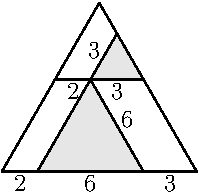
\includegraphics{J15-3}}}

\NSidePictureEPS[yoffset=-5ex,scale=0.85]{J16-2}{\problemID{16}{20272}{Greece}%
\problemRating{J}{4}{N}%
\Problem{A number is written in each of the twelve circles shown. The number inside each square indicates the product of the numbers at its four vertices. What is the product of the numbers in the eight grey circles?}
{20}{40}{80}{120}{480}
{B}{0}
{If the products inside the squares are A, B, C, D, E, then the required product is $ABDE/C^2$. This is because the numbers in grey circles are included once each at the products A, B, D and E and those in white circles show up twice each. The picture on the right shows an example with a possible construction.
\newline
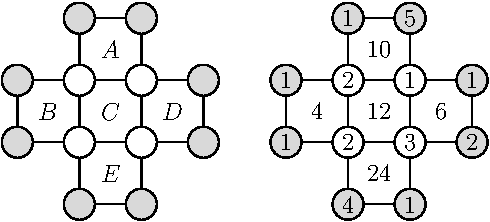
\includegraphics{J16-3}}}

\problemID{17}{20273}{Latvia}%
\problemRating{J}{4}{L}%
\Problem{There are four vases on the table in which a number of sweets have been placed.
\newline
The number of sweets in the first vase is the number of vases that contain one sweet. \newline
The number of sweets in the second vase is equal to the number of vases that contain two sweets. \newline
The number of sweets in the third vase is equal to the number of vases that contain three sweets.  \newline
The number of sweets in the fourth vase is equal to the number of vases that contain zero sweets. 
\newline
How many sweets are in all the vases together?}
{2}{3}{4}{5}{6}
{C}{0}
{If in any of the 4 vases would be more than 4 sweets that would lead to a contradiction because there are only 4 vases. If there were 4 sweets in one of the 4 vases, it would lead to a contradiction because this vase itself contains a different number of sweets. So there are only vases with 0, 1, 2 or 3 sweets. The total number of sweets is equal to the number of vases. There are at least two possible distributions in four  vases: $2,1,0,1$ or $0,2,0,2$.}

\problemID{18}{20274}{Catalonia}%
\problemRating{J}{4}{A}%
\Problem{Jean-Philippe has $n^3 (n>2)$ identical small cubes. He used these to make a large cube and painted the entire outer surface of the large cube. 

The number of small cubes with only one face painted is equal to the number of those with no face painted. What is the value of $n$?}
{4}{6}{7}{8}{10}
{D}{0}
{There are $(n-2)^2$ small cubes with a single painted face visible on each face of the large cube; so the total number is $6(n-2)^2$.  There are $(n-2)^3$ cubes without any outer face and the big cube. From  $6(n-2)^2=(n-2)^3$ and $n>2$ we deduce  $n=8$.}

\problemID{19}{20275}{Greece}%
\problemRating{J}{4}{N}%
\Problem{Cristina has a set of cards numbered 1 to 12. She places eight of them at the vertices of an octagon so that the sum of every pair of numbers at opposite ends of an edge of the octagon is a multiple of 3.

Which numbers did Cristina not place?}
{1, 5 , 9, 12 }{3, 5, 7, 9   }{1, 2, 11, 12}{  5, 6, 7, 8}{3, 6, 9, 12  }
{E}{0}
{If one of the numbers at a vertex is a multiple of 3 then the number at EVERY neighbouring vertex must also be a multiple of 3. Since we have only 4 multiples of 3 we come to a contradiction. So the numbers 3, 6, 9, 12 must be removed. \newline
2 possible constructions are given below. 
\newline
   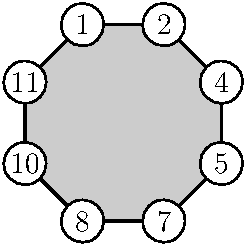
\includegraphics{J19-1}   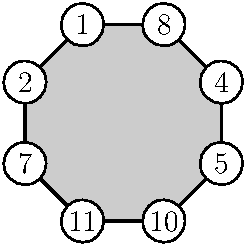
\includegraphics{J19-2}}

\NSidePictureEPS[xlines=2]{J20-1}{\problemID{20}{20276}{Mexico}%
\problemRating{J}{4}{G}%
\Problem{Otis makes a net using a combination of squares and equilateral triangles, as show in the figure. The side-length of each square and of each triangle is $1\,\textup{cm}$. He folds the net up into the 3D shape shown. What is the distance between the vertices $A$ and $B$?}
{$\sqrt{5}\ \textup{cm}$}{$(1+\sqrt{2})\ \textup{cm}$}{$\dfrac{5}{2}\ \textup{cm}$}{$(1+\sqrt{3})\ \textup{cm}$}{$2\sqrt{2}\ \textup{cm}$}
{B}{1}
{The 4 vertices joined to $A$ form a square $CDEF$ of side $1\,$cm long. Therefore, by the Pythagorean theorem, its diagonal $CE$ is $\sqrt{2}\,$cm long. Let $M$ be the midpoint of $CE$. Then $AMC$ is a right triangle with hypotenuse $AC$ of side 
$1\,$cm and leg $CM$ of side $\frac{\sqrt{2}}{2}\,$cm. Again, using the Pythagorean theorem, we get 
$$|AM|^2=1-\left(\dfrac{\sqrt{2}}{2}\right)^2=1-\dfrac{2}{4}=\dfrac{1}{2},$$ 
thus $$|AM|=\dfrac{1}{\sqrt{2}}=\dfrac{\sqrt{2}}{2}.$$
The distance between $A$ and $B$ is 
$$\dfrac{\sqrt{2}}{2}+1+\dfrac{\sqrt{2}}{2}=1+\sqrt{2}.$$
\newline
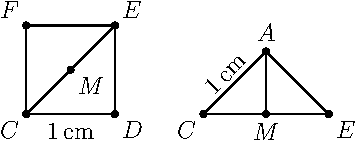
\includegraphics{J20-2}}}

\noindent\fbox{5 points}\bigskip

\problemID{21}{20277}{Greece}%
\problemRating{J}{5}{N}%
\Problem{The prime factorisation of the number $n! = 1 \cdot 2 \cdot \ldots \cdot n$ is of the form shown in the diagram.\newline
\centerline{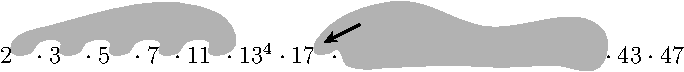
\includegraphics{J21-1}}\newline
The primes are written in increasing order. Ink has covered some of the primes and some of the exponents. What is the exponent of 17?}
{1}{2}{3}{4}{5}
{C}{0}
{The appearance of the prime 47 shows that $47 \le n < 53$ (else we would see the next prime 53).
Since $13^4$ is part of the factorization, 4 multiples of 13 are included in $n!$. These are 13, 26, 39, and 52, so $n=52$. There are three multiples of 17 before 52 (these are 17, 34 and 51). Therefore, the exponent of 17 in this factorization is 3.}

\problemID{22}{20278}{Hungary}%
\problemRating{J}{5}{L}%
\Problem{Carl always tells the truth or always lies on alternate days. One day, he made exactly four of the following five statements. Which one could he not have made on that day?}
{I lied yesterday and I will lie tomorrow.}{I am telling the truth today and I will tell the truth tomorrow.}{2024 is divisible by 11.}{Yesterday was Wednesday.}{Tomorrow will be Saturday.}
{C}{3}
{Statement (B) can only be made by a person who lies on that day. Looking at the statements (D) and (E), they cannot both be true. Therefore, we have at least two statements that are lies. This means that  Carl is lying today, so he couldn't make the statement (C).}

\problemID{23}{20279}{Russia}%
\problemRating{J}{5}{N}%
\Problem{The sum of the digits of the number $N$ is three times the sum of the digits of the number $N + 1$. What is the smallest possible sum of the digits of $N$?}
{9}{12}{15}{18}{27}
{B}{0}
{The sum of the digits of a number decreases only if the number has the last digit 9, so that the next number ends in 0, and 1 is added to its penultimate digit. In that case, the sum of the digits of the number $N+1$ decreases by 8, compared to that of the number $N$. At the same time, it is three times smaller than the sum of the digits of $N$. Denoting the sum of the digits of $N$ by $x$, we have
$$x=3(x-8)\Leftrightarrow2x=24\Leftrightarrow x=12.$$ 
Note that if the number ends in more that one 9, its sum of digits will be at least 19, which is already greater than 12.
The number 39 has the property described above.}

\problemID{24}{20280}{Austria}%
\problemRating{J}{5}{G}%
\Problem{Jill has some black, gray, and white unit cubes. She uses $27$ of them to build a $3\times 3\times 3$ cube. She wants the surface to be exactly one-third black, one-third gray, and one-third white.  The smallest possible number of black cubes she can use is $A$ and the largest possible number of black cubes she can use is $B$.  What is the value of $B - A$?}
{1}{3}{6}{7}{9}
{D}{0}
{The surface area of the cube is $6\cdot 3^2=54$. This means that the black, the grey and the white area should equal to 18 each. 
\newline
Each unit cube can contribute 3 if it is a corner cube, 2 if it is an edge cube, and 1 if it is a center of a face. 
\newline
There are 8 corner cubes, 12 edge cubes and 6 centers of faces. 1 unit cube is completely hidden from the surface. The smallest number of unit cubes to make area of 18 is $A=6$ corner cubes. The largest number of unit cubes to make area of 18 is 12: 6 centers of faces and 6 edge cubes. Indeed, we can choose the ``hidden'' unit cube to have the same color, so we would have used $B=13$ black unit cubes. In other words, $B=13,A=6, B-A=7$.
\newline
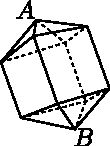
\includegraphics{J24-1}}

\problemID{25}{20281}{Catalonia}%
\problemRating{J}{5}{L}%
\Problem{Ann rolled a normal die 24 times. All numbers from 1 to 6 came up at least once. The number 1 came up more times than any other number. Ann added up all the numbers.  The total she obtained was the largest one possible.  What total did she obtain?}
{83}{84}{89}{90}{100}
{D}{0}
{Since Ann has rolled each number at least once, we can guarantee that 6 of the rolls have a sum of $1+2+3+4+5+6=21$. Let's consider the remaining 18 rolls. 
\newline
There should be more 1s than any other numbers. It is clear that the number of 6s rolled should be one less than the number of 1s.
\newline
If we have 9 1s: then 8 6s adding a 5 we get $9+48+5=62$.
\newline
If we have 8 1s: then 7 6s adding 3 5s we get $8+42+15=65$.
\newline
If we have 7 1s: then 6 6s adding 5 5s we get $7+36+25=68$.
\newline
If we have 6 1s: then 5 6s, 5 5s and adding 2 4s we get $6+30+25+8=69$. This leads to a max total of 90.
\newline
Further reduction of 1s does not increase the maximum possible sum.}

\newpage\problemID{26}{20282}{Russia}%
\problemRating{J}{5}{A}%
\Problem{Olya walked in the park. She walked half of the total time at a speed of 2 km/h. She walked half of the total distance at a speed of 3 km/h. She walked the rest of the time at a speed of 4 km/h. For what fraction of the total time did she walk at a speed of 4 km/h?}
{$\dfrac{1}{14}$}{$\dfrac{1}{12}$}{$\dfrac{1}{7}$}{$\dfrac{1}{5}$}{$\dfrac{1}{4}$}
{A}{0}
{Let's denote the half of the time for Olya's walk with $t$ and the time she walks with a speed of 4 km/h with $x$. Then, the time she walks with a speed of 3 km/h is $t-x$. We have the following:
\newline
Speed: 2 km/h, Time: $t$, Distance : $2t$ 
\newline
Speed: 3 km/h, Time: $t-x$, Distance : $3(t-x)$ 
\newline
Speed: 4 km/h, Time: $x$, Distance : $4x$ 
\newline
Then we have
$$3(t-x)=2t+4x\Leftrightarrow t=7x\Leftrightarrow x=t/7$$
Therefore, $x=1/14(2t)$. That is, $1/14$ of the time was spent walking with a speed of 4 km/h.}

\problemID{27}{20283}{Turkey}%
\problemRating{J}{5}{N}%
\Problem{Ali wants to remove some of the integers from 1 to 25 and then separate the remaining numbers into two groups 
so that the products of the integers in each group are equal. What is the smallest number of integers Ali could remove?}
{4}{5}{6}{7}{8}
{B}{0}
{Thinking of the prime factorizations of the products of the numbers of both groups, they have to be the same, since the products are equal. Therefore, prime numbers that have only one multiple among the numbers from 1 to 25 have to be removed. These prime numbers are 13, 17, 19 and 23. 7 has three multiples among the numbers from 1 to 25: 7, 14 and 21. At least one of them must be removed, which works only with the deletion of 7. The remaining 20 numbers can be split in two groups that have equal product. 
\newline
For example:
$$3\cdot5\cdot8\cdot14\cdot15\cdot18\cdot20\cdot22\cdot24=2\cdot4\cdot6\cdot9\cdot10\cdot11\cdot12\cdot16\cdot21\cdot25=2^{11}\cdot3^{5}\cdot5^3\cdot7\cdot11.$$}

\problemID{28}{20284}{Hong Kong}%
\problemRating{J}{5}{L}%
\Problem{Twenty points are equally spaced on the circumference of a circle. 
David draws all the possible chords that connect pairs of these points.  How many of these chords are longer than the radius of the circle but shorter than its diameter?}
{90}{100}{120}{140}{160}
{C}{0}
{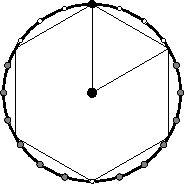
\includegraphics[scale=1.2]{J28-1}\newline
Each of the 20 points is connected with the 19 other points on the circumference, forming 19 chords. One of these 19 chords is exactly equal to the diameter, leaving 18 chords to consider. 
\newline
For a chord to be larger than the radius, its central angle has to be larger than $60^\circ$.
\newline
Since the 20 points form a regular 20-gon, the central angle of the chord connecting two adjacent points is $360/20=18^\circ$. Therefore, we need at least 4 central angles ($3\cdot18^\circ=54^\circ<60^\circ$). 
\newline
That is, 3 pairs of chords from a point to its three nearest points along the circumference (on either side) are going to be shorter than the radius. This leaves us with 6 pairs of chords, or 12 chords per point. Since each chord is counted twice (once per endpoint) the total number of chords satisfying the condition is $(20\cdot 12) : 2 = 120$.}

\problemID{29}{20285}{Belarus}%
\problemRating{J}{5}{G}%
\Problem{There are $n$ distinct lines on the plane, labeled $\ell_1, \dots, \ell_n$. The line $\ell_1$ intersects exactly $5$ other lines, the line $\ell_2$ intersects exactly $9$ other lines, and the line $\ell_3$ intersects exactly $11$ other lines. 
Which of the following is a smallest possible value of $n$?}
{11}{12}{13}{14}{15}
{B}{0}
{Since one of the lines intersects 11 other lines, the minimum number of lines is 12. On the other hand, taking a family of 7 parallel lines, another family of 3 parallel lines perpendicular to the first family and two other lines, intersecting each other and intersecting both families of parallel lines, we have an arrangement of lines that conforms to the requirement. Any of the lines in the first family of 7 parallel lines can be $\ell_1$, as it intersects 5 other lines. Any of the lines in the second family of 3 parallel lines can be $\ell_2$ as it intersects 9 other lines. Finally, any of the last two lines can be $\ell_3$ as it intersects 11 other lines. Therefore, the answer is 12.
\newline
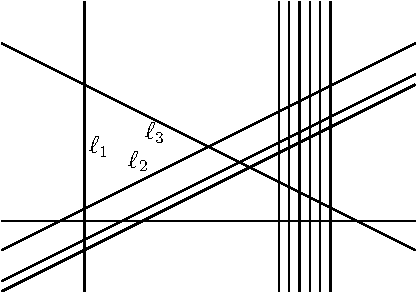
\includegraphics{J29-1}}

\NSidePictureEPS[scale=0.8]{J30-1}{\problemID{30}{20286}{China}%
\problemRating{J}{5}{N}%
\Problem{Suppose $m$ and $n$ are integers with $0<m<n$. Let $P=(m, n)$, $Q=(n, m)$, and $O=(0,0)$. For how many pairs of $m$ and $n$ will the area of triangle $OPQ$ be equal to 2024?}
{4}{6}{8}{10}{12}
{B}{0}
{$A_{\triangle OPQ}= n^{2}-mn-\frac{1}{2}(n-m)^{2}=\frac{1}{2}(n^{2}-m^{2}) = 2024 \implies (n+m)(n-m)=4048$. \newline
Since $m$ and $n$ are both integers $n+m$ and $n-m$ are both even or both odd. \newline
There are six ways that $4048=2^4\cdot 11\cdot 23$ can be represented as a product of two even numbers: $2\times 2024$, $2^2 \times 1012$, $2^3 \times 506$, $(2\cdot 11) \times (2^3\cdot 23)$, $(2^2\cdot 11)\times (2^2\cdot 23)$, $(2\cdot 23) \times(2^3\cdot 11)$, so there are 6 possible pairs of $(n,m): \{(1013, 1011),(508, 504),(257,249),(103,81),(68,24),(67,21)\}$.}}


\end{document}